\documentclass[t]{beamer}


% Appearance:

\usetheme{KTHprofile}
\usefonttheme[onlylarge]{structurebold}



% Standard packages
\usepackage{picture}
\usepackage[english]{babel}
\usepackage[latin1]{inputenc}
\usepackage{times}
\usepackage[T1]{fontenc}
\usepackage{lipsum}
\usepackage[]{epstopdf}
\usepackage[absolute,overlay]{textpos}
\usepackage{pifont}
\usepackage{subfig}
\graphicspath{{Results/}{Algorithm/}}
\newcolumntype{M}[1]{>{\arraybackslash}m{#1}}
\title[Inisintiur sequi aliquia tis dis in para] 
{%
  Safe learning for control: \\ \small{Combining disturbance estimation, reachability\\ analysis and reinforcement learning\\ with systematic exploration}%
}

%\author{}
\vspace{1cm}
\author[Oskar, Friends]
{
Caroline Heidenreich
}

%\author[Dude, Friends]
%{
%The~Dude\inst{1} \and
%And~Friends\inst{2}
%}

\institute{}

%\institute[KTH Royal Institute of Technology]
%{\inst{1} KTH Royal Institute of Technology, Sweden\and
%\vskip-4mm
%\inst{2} KTH Royal Institute of Technology, Sweden
%}

\date{\today}


\begin{document}


\begin{frame}
\titlepage
\end{frame}


\begin{frame}
\frametitle{Motivational Example}
\begin{itemize}
\item Autonomous vehicle with partly known model
\item Task: find optimal control without driving off the road
\item To simplify, we only look at the truck's position
\end{itemize}
\begin{textblock*}{5cm}(8cm,4.79cm) % {block width} (coords)
\includegraphics[width=0.29\paperwidth]{TruckOnStreet}
\end{textblock*}
\end{frame}

\begin{frame}
\frametitle{Motivation}
How can we find the optimal control?
\vspace{0.5cm}
\begin{enumerate}
\item Model-based control:
\begin{itemize}
\item Not possible without physical insight.
\end{itemize}
\vspace{1cm}
\item Learn a policy with Reinforcement Learning (RL):
\begin{itemize}
\item Directly or indirectly.
\item Requires to visit all (safe) states.
\end{itemize}
\end{enumerate}

\end{frame}

\begin{frame}
\frametitle{Motivation}
How can we make sure to stay on the road?
\vspace{0.5cm}
\begin{itemize}
\item RL algorithms not designed for satisfying constraints.
\item We need an additional safety-preserving controller.
\end{itemize}
\vspace{1cm}
$\Rightarrow$ Safe Learning Control
\end{frame}



\begin{frame}
\frametitle{Algorithm}
\framesubtitle{Markov Decision Process}
\begin{itemize}
\item Discretise states and actions.
\item Assign rewards to each state-action pair.
\item Determine objective that agent should maximise.
\end{itemize}
\begin{textblock*}{7cm}(2.3cm,5.05cm) % {block width} (coords)
\small{Reward function}\\
\includegraphics[trim=0mm 0mm 0mm 0mm, width=0.5\textwidth]{Reward}
\end{textblock*}
\begin{textblock*}{5cm}(7cm,5.05cm) % {block width} (coords)
\small{Objective function}
\end{textblock*}
\begin{textblock*}{5cm}(6.2cm,6.2cm) 
\begin{equation*}
\noindent
R_t = \sum_{k=0}^T\gamma^kr_{t+k+1}
\end{equation*}
\end{textblock*}
\end{frame}


\begin{frame}
\frametitle{Algorithm}
\framesubtitle{Reinforcement Learning}
Finding optimal policy by 
\begin{itemize}
\item play action
\item receive reward
\item update policy
\end{itemize} 
\vspace{2cm}
\ding{51} There are algorithms that converge to the optimal policy.
\ding{55} No safety guarantees.
\begin{textblock*}{18cm}(6.2cm,2cm) % {block width} (coords)
\includegraphics[trim=0mm 0mm 0mm 0mm, width=0.34\textwidth]{flow_learn_final.png}
\end{textblock*}
\end{frame}

\begin{frame}
\frametitle{Algorithm}
\framesubtitle{Safe Set Calculation}
How can we ensure safety with uncertain dynamics?
\begin{itemize}
\item Treat the unknown dynamics as bounded disturbance.
\item Determine for each state if our control manages to keep us on the road for all disturbances.
\end{itemize}

\begin{figure}
\vspace{-0.1cm}
\includegraphics[clip, trim=3mm 3mm 4mm 10mm, width=0.38\textwidth]{SafeStreet}
\end{figure}

\end{frame}

\begin{frame}
\frametitle{Algorithm}
\framesubtitle{Safe Learning}
\begin{itemize}
\item At the borders of the safe set: Apply safe control.
\item Within the safe set: Reinforcement learning.
\end{itemize}
\vspace{1cm}
\ding{51} Learn a control without leaving the road.\\
\ding{55} Small safe set due to conservative disturbance range.
\end{frame}

\begin{frame}
\frametitle{Algorithm}
\framesubtitle{Disturbance Estimation with Gaussian Processes}
\begin{itemize}
\item Update the disturbance range with measured data.
\item Gaussian Process regression: Non-parametric regression method that gives:
\begin{enumerate}[a.]
\item an estimate for the disturbance.
\item a measure how certain this estimate is.
\end{enumerate}
\end{itemize}
\begin{textblock*}{6.3cm}(3cm,5.5cm) % {block width} (coords)
\includegraphics[trim=0mm 0mm 0mm 0mm, width=0.5\textwidth]{safetyloop}
\end{textblock*}
\begin{textblock*}{9.5cm}(7cm,5.4cm) % {block width} (coords)
\includegraphics[trim=0mm 0mm 0mm 0mm, width=0.5\textwidth]{GP_idea}
\end{textblock*}
\end{frame}


\begin{frame}
\frametitle{Algorithm}
\framesubtitle{Exploration}
\begin{itemize}
\item Trade-off between exploration and exploitation.
\item Need for visiting the whole safe set i.o. to learn policy.
\item Chosen method: Promote state-action pairs that have not been visited often.
\end{itemize}
\end{frame}

\begin{frame}
\frametitle{Algorithm}
\framesubtitle{Summary of Approach}
\begin{textblock*}{11cm}(2cm,3cm) % {block width} (coords)
\includegraphics[trim=3mm 3mm 3mm 14mm, width=0.8\textwidth]{flow_final}
\end{textblock*}
\end{frame}

\begin{frame}

\renewcommand{\arraystretch}{1.3}
\frametitle{Implementation}

\begin{table}[H]
		\centering
		\makebox[\textwidth][c]{
\begin{tabular}{M{4.5cm}M{6.5cm}}
\hline \hline
Reinforcement Learning & Version of Delayed Q-learning \\
Disturbance Estimation & Gaussian Processes \\
Safe Set & Hamilton-Jacobi-Isaacs Reachability\\
Exploration & Incremental Q-learning\\ \hline \hline
\end{tabular} }
\end{table}
\vspace{0.6cm}
Evaluate approach on:
\begin{itemize}
\item Inverted Pendulum System.
\item Two states: position and angular velocity.
\item Four iterations with 10,000 learning steps.
\end{itemize}
\begin{textblock*}{4cm}(10cm,5.2cm) % {block width} (coords)
\includegraphics[trim=0mm 0mm 0mm 0mm, width=0.5\textwidth]{Pendulum}
\end{textblock*}
\end{frame}

\begin{frame}
\frametitle{Experimental Results}
\framesubtitle{Exploration}

\begin{textblock*}{8cm}(0cm,3cm) % {block width} (coords)
\includegraphics[width=0.8\textwidth]{Unexploration_samples}
\end{textblock*}
\begin{textblock*}{8cm}(6cm,3cm) % {block width} (coords)
\includegraphics[width=0.8\textwidth]{Exploration_samples}
\end{textblock*}
\end{frame}



\begin{frame}
\frametitle{Experimental Results}
\framesubtitle{Policy Estimation}

\begin{figure}
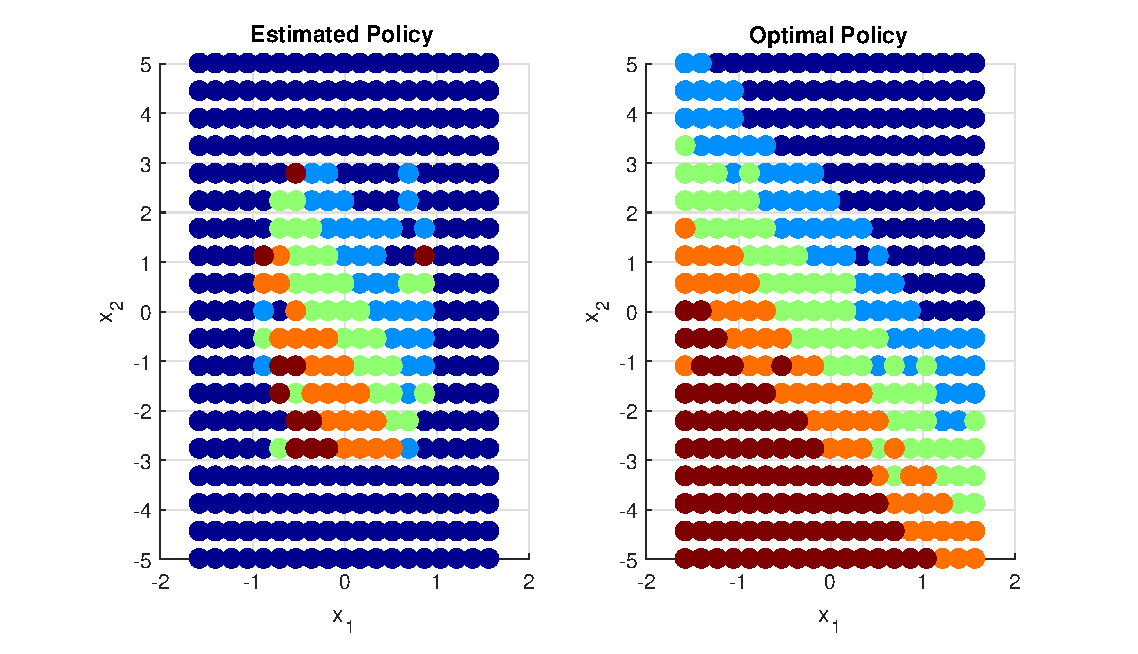
\includegraphics[width=0.8\paperwidth]{Policy}
\end{figure}
\end{frame}

\begin{frame}
\frametitle{Experimental Results}
\framesubtitle{Disturbance Estimation}

\begin{figure}[width=\paperwidth]
  \makebox[\linewidth][c]{%
  \centering
  \uncover<1->{\subfloat{\includegraphics[height=2.7cm,width=6cm]{GP_1_1}}}%
  \uncover<3->{\subfloat{\includegraphics[height=2.7cm,width=6cm]{GP_1_2}}}%
  }
  \makebox[\linewidth][c]{%
  \uncover<2->{\subfloat{\includegraphics[height=2.2cm,width=6cm]{GP_2_1}}}%
  \uncover<4->{\subfloat{\includegraphics[height=2.2cm,width=6cm]{GP_2_2}}}%
  }
\end{figure}
\end{frame}

\begin{frame}
\frametitle{Experimental Results}
\framesubtitle{Trajectories}
\begin{figure}
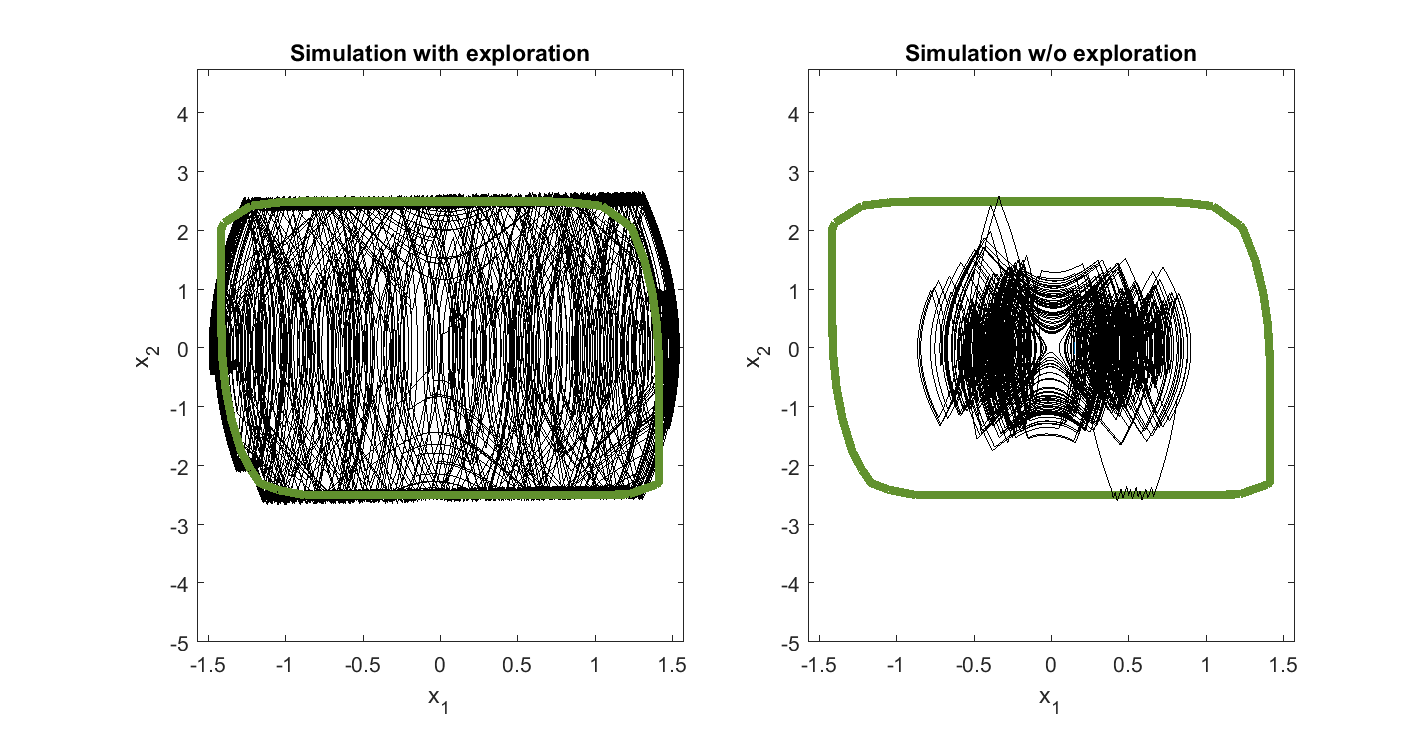
\includegraphics[width=0.8\paperwidth]{Simulation}
\end{figure}
\end{frame}

\begin{frame}
\frametitle{Experimental Results}
\framesubtitle{Trajectories}
\begin{textblock*}{12cm}(1cm,3cm) % {block width} (coords)
{\includegraphics[width=\textwidth]{switch_title}}
\only<1>{\includegraphics[width=\textwidth]{switch_upper}}
\only<2>{\includegraphics[width=\textwidth]{switch_middle}}
\only<3>{\includegraphics[width=\textwidth]{switch_lower}}
\end{textblock*}
\end{frame}



\begin{frame}
\frametitle{Conclusions}
\begin{itemize}
\item We manage to learn an accurate policy for inverted pendulum.
\item System can always be brought back to safety.
\item Considerably better results by incorporating exploration.
\end{itemize}

\end{frame}

\begin{frame}
\frametitle{Future Work}
Some theoretical \& practical challenges remain:
\begin{itemize}
\item Joint design of safety and learning loop.
\item Recursive estimation of disturbance bounds.
\item Formal guarantees for the whole algorithm.
\makebox(1,1.1){\put(1,2\normalbaselineskip){%
               $\left.\rule{0pt}{1.2\normalbaselineskip}\right\}$ theoretically}}
\begin{textblock*}{2cm}(10.5cm,4cm) % {block width} (coords)
challenging
\end{textblock*}
\end{itemize}
\end{frame}

\begin{frame}
\vspace{1cm}
\huge{Thank you for listening!}\\
\vspace{2cm}
\huge{Questions?}
\begin{textblock*}{5cm}(8cm,4.79cm) % {block width} (coords)
\includegraphics[width=0.29\paperwidth]{TruckOnStreet}
\end{textblock*}
\end{frame}
\end{document}